\chapter{Wiring and Setup}
\label{sec:setup}

In this appendix, I briefly go through the critical components of the wiring of a dilution refrigerator.
Throughout my Ph.D., I have been lucky enough to see the lab grow from one to seven fridges. This has given me
plenty of opportunities to optimize the wiring of a refrigerator to minimize the electron temperatures seen by
devices. It has also allowed me to test a large selection of hardware and confirm that it does or does not work
cold. The fridge wiring I present in Fig.~\ref{fig:wiring} is a setup optimized for operation on spin qubits, however,
for other types of experiments, the values of the attenuators and filtering may be tweaked to trade-off heating and thermal
photon population~\cite{Krinner2019}.

\begin{figure}
    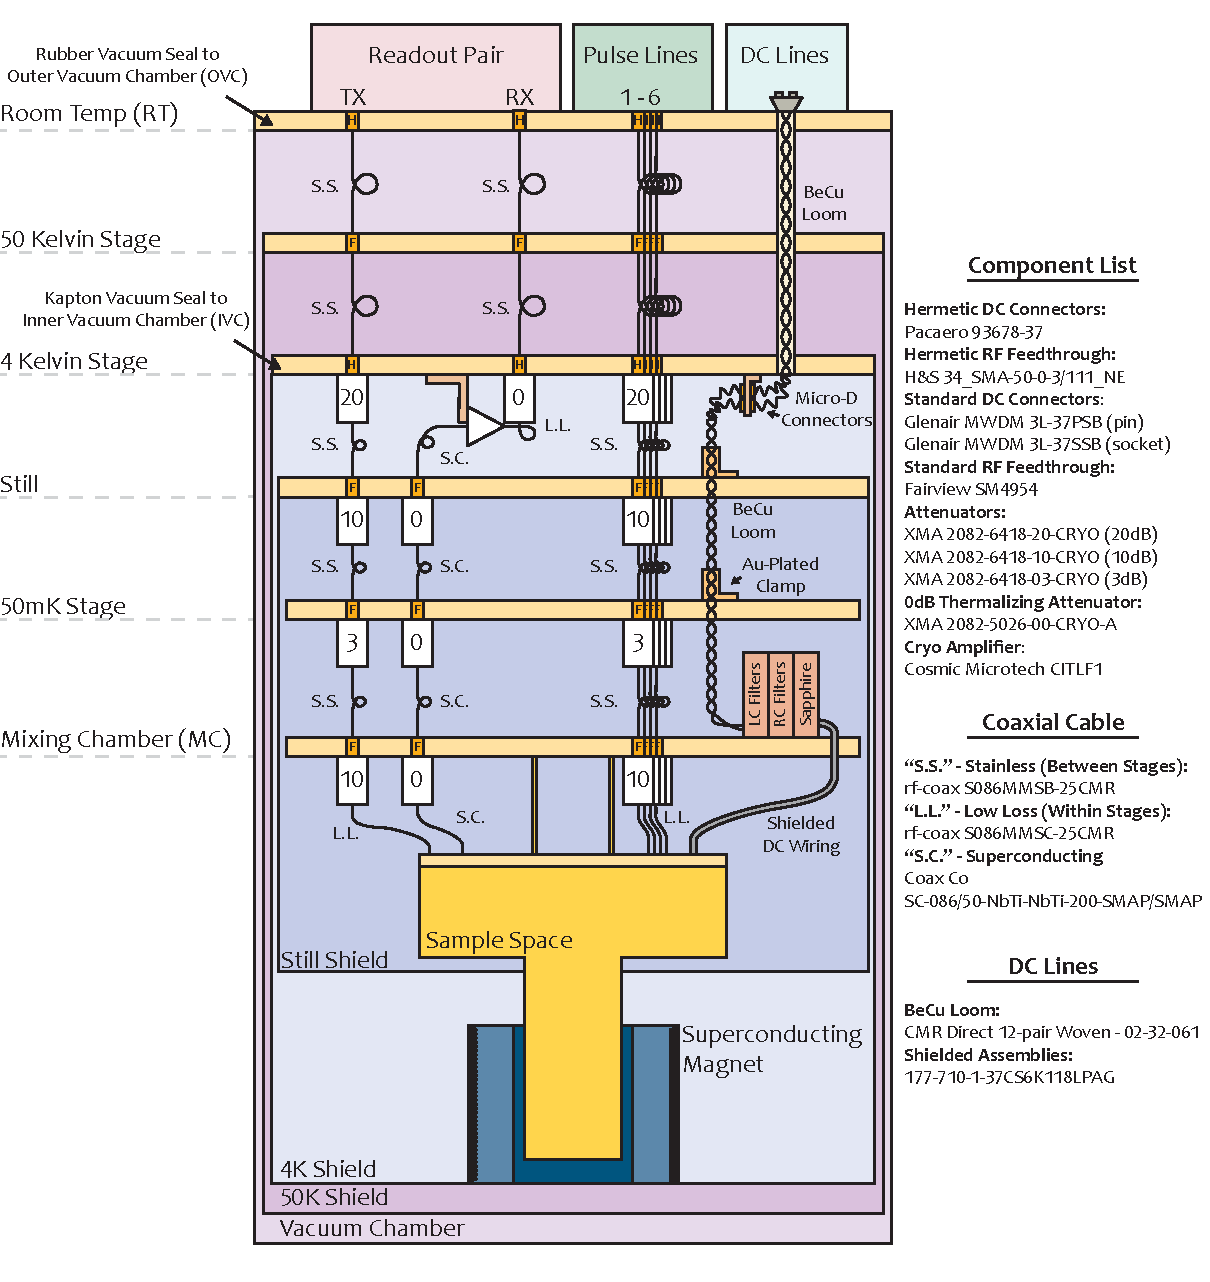
\includegraphics[width=\linewidth]{Setup}
    \caption[Standard wiring diagram for a dilution refridgerator]
    {\label{fig:wiring}The standard fridge wiring for a spin qubit experiment. Values for attenuators are chosen to trade-off power dissipation from pulses and the thermal photon population. Components which are known to work cryogenically are given on the right of the figure, although the list is by no means exhaustive.}
\end{figure}

High-frequency coaxial lines are used in both the readout circuit and for pulsing qubits. These are fed into
the fridge with Huber $\&$ Suhner hermetic feedthroughs, rated to \SI{18}{\giga\hertz} (H $\&$ S 34\_SMA-50-0-3/111\_NE),
and are in my experience the highest quality hermetic connectors around. On the 4K stage, as the o-ring will pass
through its transition temperature, the connectors must be soldered into place, or run down a dedicated port
directly into the inner vacuum chamber. On BlueFors or Oxford fridges where there is no inner vacuum chamber,
this is not an issue.

For most fridges that we've wired ourselves, we've used 0.086-inch diameter coax, with differing inner and outer
conductors depending on the location. Between temperature stages, the choice of material for coaxial cables is
crucial to minimize heat transfer. In my experience, a stainless steel outer with a beryllium-copper inner conductor is
sufficiently insulating (UT-085-B-SS), although stainless steel inner conductor coax is available and used on some
setups (UT-085-SS-SS). Premade cable assemblies are generally more reliable and can be ordered from rf-coax or Rojone,
(see for example the part numbers given in Fig.~\ref{fig:wiring}). In the case that manual assembly is required,
the Radiall 9401-1583-010 SMA connectors do not require soldering of the inner contact and are highly reliable. On
readout lines where any attenuation of the signal leads to an increased noise temperature
(see Sec.~\ref{sec:readout}), superconducting coaxial lines are used. Soldering NbTi is unfortunately almost
impossible; in this case, premade assemblies are used exclusively. These are available from CoaxCo and
have a narrow \SI{0.85}{\milli\meter} diameter. Part number (SC-086/50-NbTi-NbTi-200-SMAP/SMAP) is commonly
ordered and is a \SI{20}{\centi\meter} SMA male to SMA male assembly.

In terms of attenuators, we have begun using only XMA corp cryogenic attenuators, part no. 2082-6418-XX-CRYO,
where XX is replaced with the required attenuation. These are used on each temperature stage to thermalize
the inner contact through the resistive link (which would otherwise make no contact to each temperature stage) and
reduce the population of thermal photons. Again for readout lines, where losses must be minimized, XMA corp
\SI{0}{\decibel} attenuators are used (2082-5026-00-CRYO-A), which contain a thermally conductive stripline to
thermalize the inner conductor.

The amplifiers we use are either SiGe resistive feedback amplifiers from Cosmic Microwave (formerly the Weinreb group
at Caltech) or amplifiers from Low Noise Factory. The CITLF1 or CITLF3 from Cosmic Microwave are used interchangeably in
low-frequency experiments, while in transmon-type experiments typically use a Low Noise Factory amplifier. All of these amplifiers
have $\sim \SI{4}{\kelvin}$ noise temperature in their respective operating frequency ranges.

\begin{figure}
    \includegraphics[width=\linewidth]{dc}
    \caption[DC thermalization]
    {\label{fig:dc}(a) A thermalization clamp used on each temperature stage of the dilution refrigerator. BeCu loom wire is wrapped and clamped between the two plates. (b) An image of the assembled dc filtering setup. Each stage is labeled. Input and output occur via Micro-D connectors. (c) Disassembled RC filter stage. Green boxes highlight struts used to isolate each stage of the filter. (d) Disassembled sapphire filter stage. The sapphire chip is mounted in the center of the block and connected to PCBs at either end by bond-wires. (e) Zoom in of one corner of the sapphire filter. Here a meandering Ti/Au track is visible, as well as the ends of bond-wires
    used to connect it to the PCB.}
\end{figure}

DC lines are typically BeCu loom wire from CMR-direct. Lines are clamped at each temperature stage and are optionally
covered in GE-varnish to improve thermal contact. An image of such a clamp is shown in Fig.~\ref{fig:dc} (a). Filtering
of dc lines is performed on the mixing chamber and consists of three stages. The first two stages, an LC and RC filter,
are used to remove any high-frequency noise, as shown in Fig.~\ref{fig:dc} (c). This is followed by a sapphire stripline
filter, as shown in Fig.~\ref{fig:dc} (d). A Ti/Au meander line is fabricated on a sapphire chip and is used
to reduce the electron temperature to $\sim \SI{50}{\milli\kelvin}$, based on designs from the Marcus lab at Harvard.
A zoom-in of the track is shown in Fig.~\ref{fig:dc} (e). Component values for the LC and RC filter boards are shown in
Table~\ref{tab:filt}.

\begin{table}
    \centering
    \begin{tabular}{lll}
    \toprule
     & LC Filter & RC Filter \\
    \midrule
    Stage 1 & Minicircuits LFCN-5000 & Minicircuits LFCN-80\\
    Stage 2 & Minicircuits LFCN-1450 & R = \SI{500}{\ohm}, C = \SI{2200}{\pico\farad} \\
    Stage 3 & Minicircuits LFCN-80 & R = \SI{1200}{\ohm}, C = \SI{1000}{\pico\farad} \\
    \bottomrule
    \end{tabular}
    \caption[Component values for dc filers]{Component values for dc filtering. The LC filter has a cutoff of \SI{80}{\mega\hertz}, while the RC filter
    has a cutoff of $\sim \SI{70}{\kilo\hertz}$.}
    \label{tab:filt}
  \end{table}
